\chapter{Flyback converter}
The study model includes, in addition to the transistor control circuit, the following setup:

\begin{figure}[h]
\centering
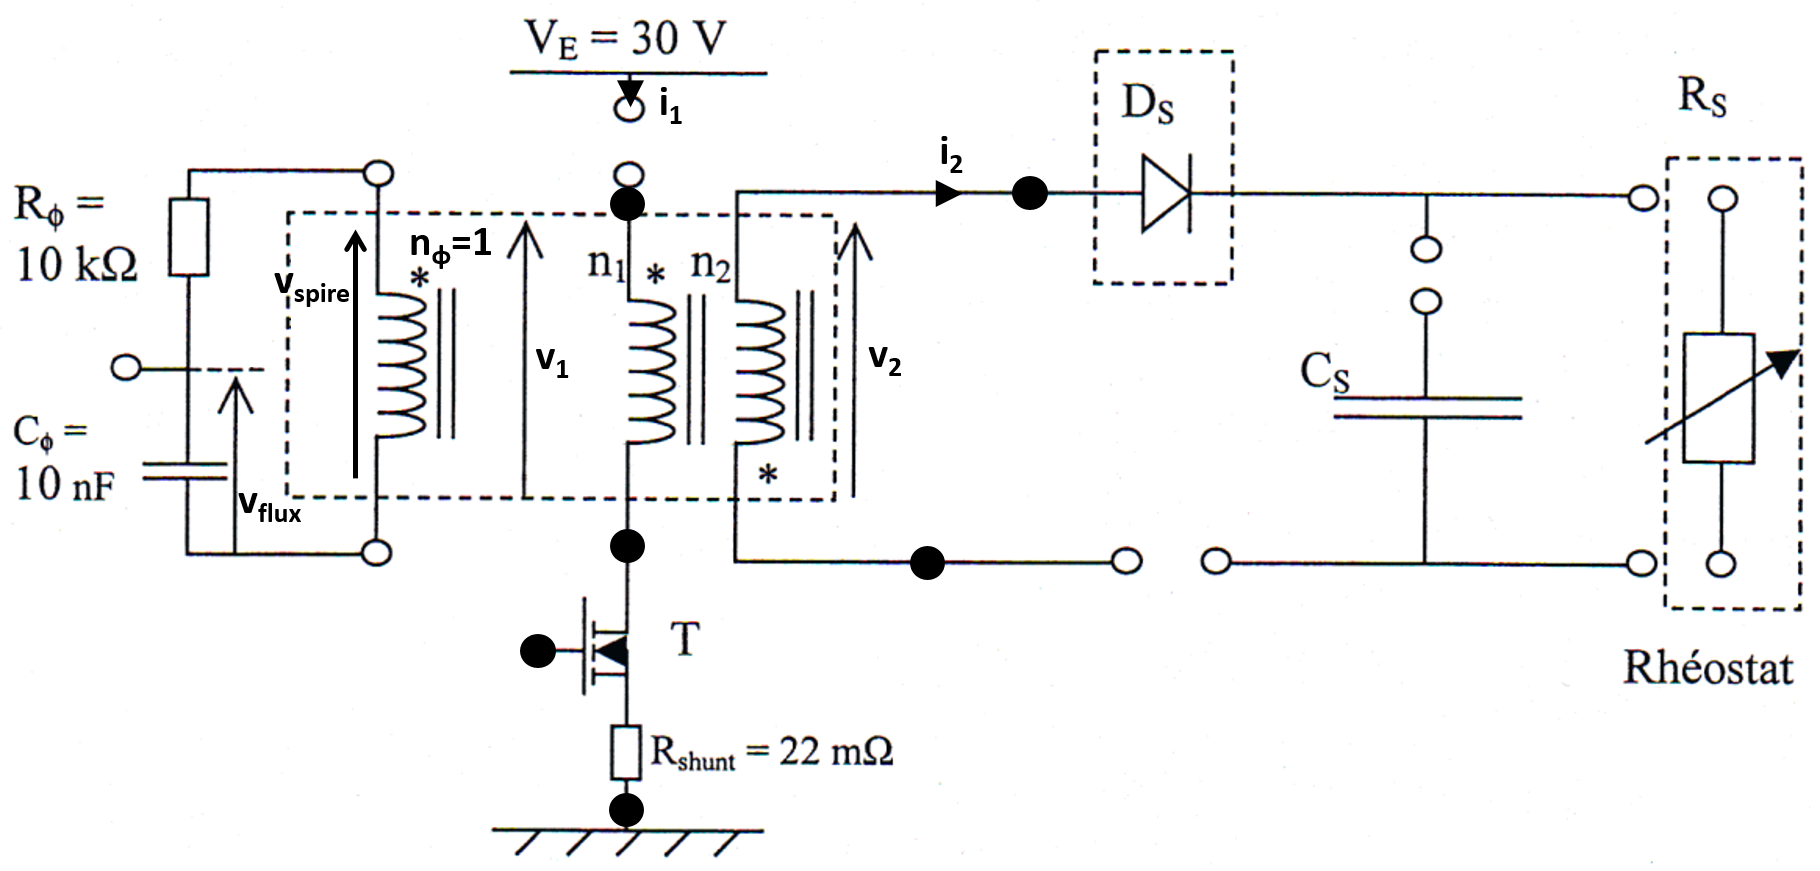
\includegraphics[width=\linewidth]{TP_Flyback/fig/Schema_Flyback.png}
%\caption{Simplified internal control}
\end{figure}

Test points $\bullet$ allow visualization of various signals, particularly the MOSFET transistor control signal.

The 3 windings are on the same ETD29/16/10 magnetic core made of N27 type ferrite, whose documentation is attached. This core can be equipped with an adjustable air gap using non-magnetic shims. In this case, the relationship between the thickness $s$ of the air gap and the specific inductance value $A_L$ is given by the following relation where $K_1$ and $K_2$ are two constants provided in the documentation:
$$s=(\dfrac{A_L}{K_1})^{\dfrac{1}{K_2}}$$

The missing connections should be made using "jumpers" to visualize the currents using appropriate probes. The load rheostat can be either 250 $\Omega$ or 330 $\Omega$ interchangeably, and care should be taken to \underline{\textbf{not connect the voltage $V_E$ without the presence}} \underline{\textbf{of this load}}.

Note the presence of a flux measurement circuit made with a single turn connected to an R-C integrator circuit. The voltage $v_{flux}$ thus allows visualization of the flux ripple in the magnetic circuit.

\newpage
The transistor control device is shown in the figure below:

\begin{figure}[h]
\centering
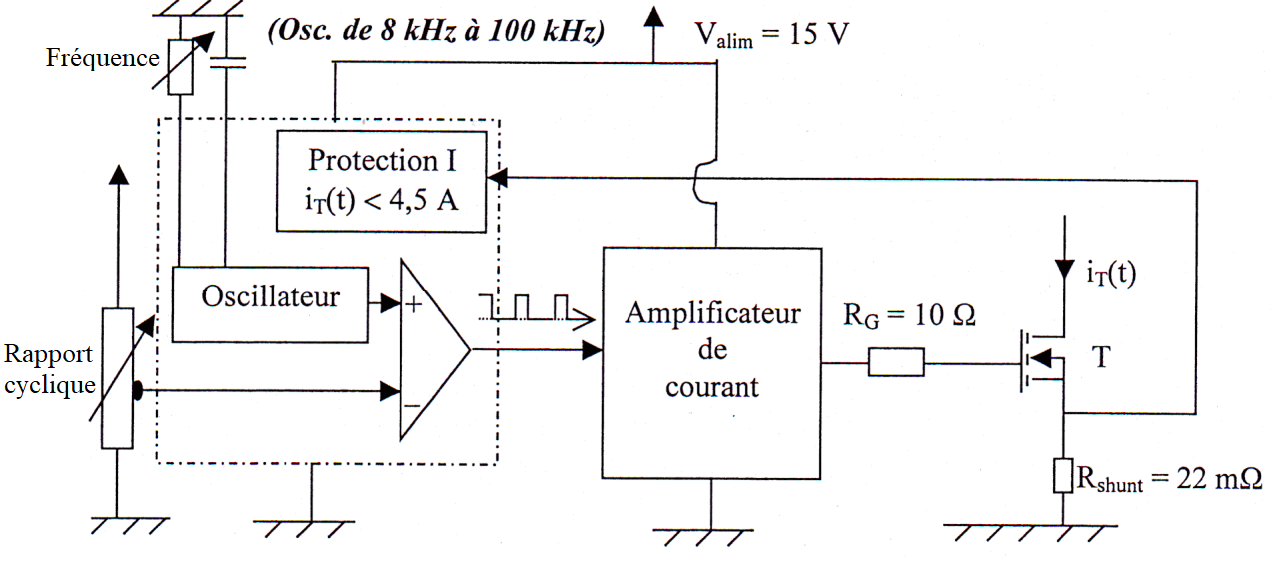
\includegraphics[width=\linewidth]{TP_Flyback/fig/Control_Flyback.png}
%\caption{Simplified internal control}
\end{figure}

A potentiometer allows adjusting the frequency (do not go below 15 kHz), and a second one allows adjusting the duty cycle. The latter is equipped with an active current limitation set at 4.5A, achieved by measuring the voltage across a 22 m$\Omega$ shunt. The power supply for this control is provided by an independent voltage source of $V_{alim} = 15 V$.

\newpage
\section{Preparation}

Assume the transistor is controlled by a PWM signal with a duty cycle $\alpha=0.25$. Also, assume that the converter operates in \textbf{total demagnetization mode} for the transformer. The input voltage $V_E$ is assumed constant. For the preparation, only the \underline{steady state} will be studied.

\begin{enumerate}
\item Complete the timing diagrams below by plotting:
\begin{itemize}
\item the flux $\varphi$ in the transformer
\item the current $i_1$ supplied by the power source
\item the current $i_2$ in the diode
\item the voltage $v_2$ at the transformer output
\end{itemize}

\begin{figure}[h]
\centering

\includegraphics[width=0.7\linewidth]{TP_Flyback/fig/prepa.png}
%\caption{Simplified internal control}
\end{figure}

\item Assume the time constant of the $R_\phi-C_\phi$ filter is much larger than the switching period of the chopper. Show that $v_{flux}$ allows visualization of the flux ripple in the transformer. Determine the flux ripple $\Delta \varphi$ as a function of $\alpha$, $T$, and the value of $v_{spire}$ over the interval $0<t<\alpha T$.
\end{enumerate}

%%%%%%%%%%%%%%%%%

\newpage
Throughout the lab session, the following precautions should be taken:

\begin{itemize}
\item use two independent sources to provide $V_{alim}$ and the "power" supply $V_E$: \textbf{carefully set the current limit of the latter to 2 A}
\item keep the $V_{alim}$ voltage present throughout the session but lower the $V_E$ voltage at each connection modification
\item do not lower the switching frequency below 15 kHz
\item when multiple voltage measurements are made simultaneously with a voltage probe, \textbf{be careful not to create a short circuit}. Indeed, the voltage probes are not isolated from each other, so the potential references of the probes are linked via the oscilloscope
\end{itemize}

\section{Magnetic Study, Waveforms}

The following measurements will be made with the load rheostat at its maximum value (reduced load) and ensuring operation in total demagnetization mode, for a duty cycle close to its maximum value.

\begin{enumerate}
\item Set the switching frequency to 50 kHz and the duty cycle to its maximum value (which will be noted). Observe the voltage across the flux measurement turn $v_{spire}$ as well as the voltage $v_{flux}$. Deduce the peak-to-peak excursion $\Delta B$ of the magnetic induction in the circuit using the documentation ($\Delta B = B_{max} – B_{min}$).
\item By comparing the voltages $v_{spire}$ and $v_1$, then $v_2$, determine the number of turns $n_1$ and $n_2$.
\item Simultaneously observe the currents $i_1$ and $i_2$ and compare them to the flux evolution.
\item Deduce the value of the primary magnetizing inductance, noted $L_1$.
\item From the measurements of $n_1$ and $L_1$ and using the documentation, determine the specific inductance value $A_L$ and the thickness of the air gap. What is the role of this air gap?
\end{enumerate}

\newpage
\section{Static Curves}

The purpose of these measurements is to plot the network of static characteristics at the output of the power supply. The switching frequency is initially kept constant at 50 kHz.

\begin{enumerate}
\item For several values of the duty cycle (e.g., $\alpha_{max}$, 0.3, 0.2, and 0.1), modify the load rheostat resistance to vary the average current supplied between its minimum value (obtained with the rheostat at maximum) and a maximum value of 2 A. Record the average values of the current supplied by the power source $V_E$, $I_E$, the output current $I_S$, and the output voltage $V_S$. Carefully note the operating point corresponding to the change in the power supply's demagnetization regime.
\item Deduce the plot of the characteristics $V_S(I_S)$ and $P_S(I_S)$ (output power) parameterized by $\alpha$. Also plot the power transfer characteristics $P_S(P_E)$ and deduce the efficiency. Highlight the operating zones in partial demagnetization and total demagnetization.
%\item To maintain the power supply in critical mode, it is possible to modify the switching frequency. This is generally done using a self-oscillating control, but this operation can be simulated as follows: set the switching frequency to maintain the average output voltage constant while the duty cycle remains constant, set to $\alpha_{max}$, for different values of the load rheostat. To easily perform these measurements, proceed "in reverse" by first setting a switching frequency value and then modifying the rheostat value to obtain the desired output voltage, e.g., $V_S = 40 V$. Record the operating point, i.e., the average output current $I_S$ and the switching frequency.

%\item Observe the waveforms of the voltage $V_{CE}$ across the transistor and the current $i_1$ through it. Deduce the constraints on the transistor.
\end{enumerate}

\section{Additional Measurements}

Keep the load rheostat at its maximum value and the switching frequency at 50 kHz.

\begin{enumerate}
\item Simultaneously observe the current $i_1$ and the voltage across the transistor $v_T$. Deduce the constraints on this transistor.% and evaluate its switching and conduction losses.
\item Simultaneously observe the current in the filter capacitor $I_{CS}$ and the output voltage $v_S$. Deduce the value of the filter capacitor $C_S$.
\end{enumerate}